\section{Prototyp-Verifikation
\label{section:verification}}
Um die Funktionalität des Prototyps zu verifizieren, wurden insgesamt sechs
separate Messungen durchgeführt. Diese Messungen beinhalten - abgesehen von 
einer Messung - alle merhere Mobilgeräte. Die Messparameter und der Verwendungszweck
sind in den nachfolgenden Unterabschnitten beschrieben.

\subsection{Messungen für die Verifikation}
\subsubsection*{Fairphone Gemischt Aktiv/Passiv}
In der 30-Minütigen Messung wurde in einem fünf-Minuten-Intervall zwischen 
aktivem und passivem verhalten auf dem Fairphone 3+ gewechselt.
Mit diesen Messdaten wurde überprüft, ob der Prototyp in der Lage ist, 
Geräte zu erkennen, die während der Probe-Request-Aufzeichnung zwischen Aktiv/Passiv 
wechseln.

Die Prototyp-Verifikation hat gezeigt, dass der Prototyp Geräte, 
die unterschiedliche IE-Felder im aktiven oder passiven Modus verwenden, 
als zwei separate Geräte klassifiziert. Eine Auswertung der verwendeten 
IE-Felder hat gezeigt, dass ausser dem Fairphone 3+ alle Geräte mehrheitlich 
die gleichen IE-Felder im aktiven wie auch im passiven Modus verwenden.

Die Abbildung~\ref{figure:fairphonemixed} zeigt das Resultat des Prototypen 
für die Messung.

\begin{figure}[h!]
	\centering
	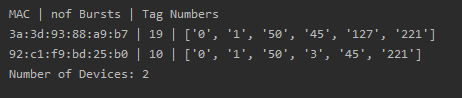
\includegraphics[width=0.75\linewidth]{Prototype/fairphone_gemischt_verifikation.PNG}
    \caption{Ausgabe des Prototyps für die Messung 
	\label{figure:fairphonemixed}}
\end{figure}

\clearpage 


\subsubsection*{Fairphone iPhone Aktiv}
In der 30-Minütigen Messung wurden Probe-Requests des iPhone X und des 
Fairphone 3+ im aktiven Modus aufgezeichnet. 
Mit den Messdaten wurde überprüft, ob der Prototyp zwischen einem 
Android- und einem iOS-Gerät unterscheiden kann.

Der Prototyp konnte in dieser Messung das Fairphone 3+ vom iPhone X unterscheiden,
wie die Abbildung~\ref{figure:fairphoneiphoneactive} zeigt.

\begin{figure}[h!]
	\centering
	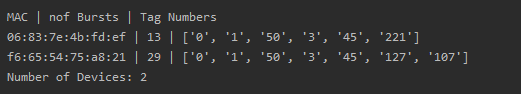
\includegraphics[width=0.75\linewidth]{Prototype/Fairphone_iphone_aktiv_verifikation.PNG}
    \caption{Ausgabe des Prototyp für die Messung 
	\label{figure:fairphoneiphoneactive}}
\end{figure}


\subsubsection*{Fairphone iPhone Passiv}
In der 30-Minütigen Messung wurden Probe-Requests des iPhone X und des 
Fairphone 3+ im passiven Modus aufgezeichnet. 
Mit den Messdaten wurde überprüft, ob der Prototyp zwischen einem 
Android- und einem iOS-Gerät unterscheiden kann.

In der Passivmessung ist nur ein Burst des Fairphone aufgetreten und der 
Prototyp hat diese falsch als Störeinfluss klassifiziert und 
nicht beachtet.
Man kann in der Abbildung~\ref{figure:fairphoneiphonepassiveone} sehen, 
dass nur ein Gerät erkannt wird.

\begin{figure}[h!]
	\centering
	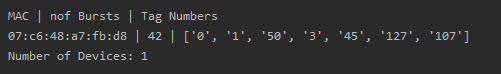
\includegraphics[width=0.75\linewidth]{Prototype/Fairphone_iphone_passiv_2_verifikation.PNG}
    \caption{Ausgabe des Prototyp für die Messung 
	\label{figure:fairphoneiphonepassiveone}}
\end{figure}

Man kann im Prototyp einstellen, wieviele Bursts in einer Liste vorkommen müssen, 
damit die Liste als separates Gerät gespeichert wird.
Man sieht in Abbildung~\ref{figure:fairphoneiphonepassivetwo} das Resultat, wenn ein Burst ausreicht, 
damit die Liste als Gerät akzeptiert wird.

\begin{figure}[h!]
	\centering
	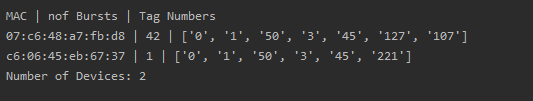
\includegraphics[width=0.75\linewidth]{Prototype/Fairphone_iphone_passiv_1_verifikation.PNG}
    \caption{Ausgabe des Prototyp für die Messung 
	\label{figure:fairphoneiphonepassivetwo}}
\end{figure}

\clearpage 

\subsubsection*{Pixel iPhone S20 Aktiv}
In der 60-Minütigen Messung wurden Probe-Requests des Google Pixel 3, des iPhone X
und des Samsung Galaxy S20+ im aktiven Modus aufgezeichnet.
Mit den Messdaten wurde überprüft, ob der Prototyp zwischen dreien Geräten 
unterscheiden kann.

Der Prototyp kann in der Messung erfolgreich die drei Geräte klassifizieren.
Die Abbildung~\ref{figure:threephonesactive} zeigt die Ausgabe des Prototyps. 

\begin{figure}[h!]
	\centering
	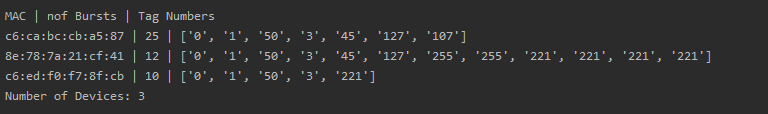
\includegraphics[width=0.75\linewidth]{Prototype/Pixel_iPhone_S20_aktiv_verifikation.PNG}
    \caption{Ausgabe des Prototyp für die Messung 
	\label{figure:threephonesactive}}
\end{figure}


\subsubsection*{Pixel iPhone S20 Passiv}
In der 60-Minütigen Messung wurden Probe-Requests des Google Pixel 3, des iPhone X
und des Samsung Galaxy S20+ im passiven Modus aufgezeichnet.
Mit den Messdaten wurde überprüft, ob der Prototyp zwischen dreien Geräten 
unterscheiden kann.

Auch in der Passivmessung wurden alle drei Geräte korrekt klassifiziert,
wie in der Abbildung~\ref{figure:threephonespassive} ersichtlich.

\begin{figure}[h!]
	\centering
	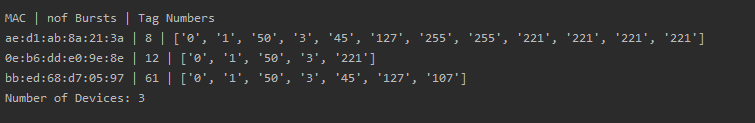
\includegraphics[width=0.75\linewidth]{Prototype/Pixel_iPhone_S20_passiv_verifikation.PNG}
    \caption{Ausgabe des Prototyp für die Messung 
	\label{figure:threephonespassive}}
\end{figure}

\clearpage 

\subsubsection*{Sechs Mobilgeräte Gemischtes Verhalten}
In dieser Messung wurden 20 Minuten lang Probe-Requests von sechs verschiedenen
Mobilgeräten aufgezeichnet. Dabei wechseln die Mobilgeräte zwischen Aktiv/Passiv, 
verbinden sich zwischendurch mit einem WLAN oder werden in den Flugmodus geschaltet.
Die Messung soll in einem kleineren Rahmen das Verhalten von Passagieren in einem 
Zug simulieren und dient der Verifikation des Prototyps mit realistischen Messdaten.

Der Prototyp erkennt acht verschiedene Geräte in der Messung.
Dies kann damit erklärt werden, dass ein Gerät je nachdem, ob es Aktiv oder Passiv ist,
separat erkannt und klassifiziert wird, wie bereits mit der Messung des Fairphone 3+ 
gezeigt. 
In der Abbildung~\ref{figure:allthephones} ist die Ausgabe des Prototyp ersichtlich.

\begin{figure}[h!]
	\centering
	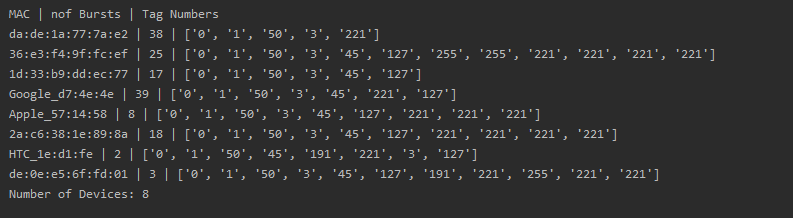
\includegraphics[width=0.85\linewidth]{Prototype/All_the_phones_realistic_verification.PNG}
    \caption{Ausgabe des Prototyp für die Messung 
	\label{figure:allthephones}}
\end{figure}

Weiterhin ist es nicht ausgeschlossen, dass ein Gerät von ausserhalb der Messkammer
aufgezeichnet wurde, da in den Versuchen kein HTC-Gerät verwendet wurde. 

\clearpage


